\documentclass[paper=letter, fontsize=15pt]{article} % For LaTeX2e
\usepackage{nips14submit_e,times}
\usepackage{hyperref}
\usepackage{url}
\usepackage{graphicx}
%\documentstyle[nips14submit_09,times,art10]{article} % For LaTeX 2.09


\title{Search Engine for Local and Global Businesses \\ SAM ! }


\author{
Suraj Swaminathan \\
Courant Institute\\
New York University \\
\texttt{ss7359@nyu.edu} \\
\And
Arpit Jain \\
Courant Institute\\
New York University \\
\texttt{arpitjain@nyu.edu} \\
\And
Mark Ward \\
Courant Institute \\
New York University \\
\texttt{maw627@nyu.edu} \\
}

% The \author macro works with any number of authors. There are two commands
% used to separate the names and addresses of multiple authors: \And and \AND.
%
% Using \And between authors leaves it to \LaTeX{} to determine where to break
% the lines. Using \AND forces a linebreak at that point. So, if \LaTeX{}
% puts 3 of 4 authors names on the first line, and the last on the second
% line, try using \AND instead of \And before the third author name.

\newcommand{\fix}{\marginpar{FIX}}
\newcommand{\new}{\marginpar{NEW}}

\nipsfinalcopy % Uncomment for camera-ready version

\begin{document}


\maketitle

\begin{abstract}
Many users now-a-days look for local businesses or places to dine at on the web. With access to a lot of data online, one can go online and search for businesses and read about not only the service provided by the business but also experiences of people who have interacted with them. We have built a search engine that makes it easier for one to find businesses locally based on reviews and ratings provided by their respective customers. We not only provide businesses that a user is looking for, but also recommend other such businesses that the user might like. 

In this report we talk about the design and implementation of the system. We briefly discuss the different ranking heuristics applied to improve the search results. We also present the evaluations conducted to judge the system performance. 
\end{abstract}

\section{Motivation}

Searching for businesses online has become easier now-a-days. Search engines such as Yelp \cite{yel} provide users with information about businesses and also opinions of people who have used services provided by the business. Ratings and reviews go a long way in determining the success of a business and people invest considerable amount of time providing their experiences and suggestions as to how could one leverage the business' services to get a positive experience. Our main aim is to make use of this user-generated information to further enhance the information retrieved by our search engine. 


We leverage information about businesses and users to build a search engine that not only searches businesses queried by our users but also recommends similar businesses in and around the vicinity of their searches. This similarity is derived from the reviews provided for each business. We used the Map-Reduce\cite{smap} framework to get the user-based and the content based similarities. The subsequent sections provide detailed discussions on how we incorporated recommendations into our search engines. The search engine also performs location based personalization such that the retrieved businesses pertain to the region our search engine is being queried from.
We have built our search engine such that one could not only use it for searching for a specific business but also use free text to look for businesses that provide services which match the user's queries. For example, one could look for places that serve pizza by querying \textit{pizza} on our search engine. 

The report is structured as follows. Section 2 talks about the basic architecture of the system and the design considerations. Section 3 discuss the implementation details. The results and evaluation of the system are provided in Section 4 and Section 5 concludes the report.


\section{Design and Architecture}
We first discuss the dataset used to generate the index for the search engine in 2.1.

\subsection{Dataset}

Our system uses Yelp's data. We gathered three different datasets from Yelp and merged them. The three dataset are following
\begin{itemize}
\item Yelp academic dataset
\item Yelp challenge dataset ( March 2015 )
\item Yelp challenge dataset ( November 2015 )
\end{itemize}
The academic dataset includes business near 30 schools in USA including Columbia University and Cornell University form New York state.
Both the challenge datasets are mainly from Phoenix, Las Vegas, Madison, Waterloo and Edinburgh, however there are many non-overlapping business in both.
The datasets are divided into majorly four parts
\begin{itemize}
\item Business
\item Review
\item Tips
\item User
\end{itemize}
Each part of the dataset is provided as a separate JSON file. We merged the information provided in the 4 json files into one text file for each business and incorporated data for over 55,642 Businesses, 1.9 million review and 403,210 tips. Table 1-4 summarizes the important fields pertaining to each dataset-part which we have used for creating the index.

\begin{table}[h!]%
\begin{minipage}{.5\linewidth}
\centering
\begin{tabular}{|l|}
\hline
\textbf{Business} \\\hline
business id\\\hline
name\\\hline
neighborhoods\\\hline
full address\\\hline
city\\\hline
state\\\hline
latitude\\\hline
longitude\\\hline
stars\\\hline
review count\\\hline
photo url\\\hline
categories\\\hline
url\\\hline
\end{tabular}
\caption{Important Attributes for Business }
\end{minipage}
\label{}
\begin{minipage}{.5\linewidth}
\centering
\begin{tabular}{|l|}
\hline
\textbf{Review} \\\hline
business id\\\hline
user id\\\hline
stars\\\hline
text\\\hline
date\\\hline
votes\\\hline
\end{tabular}
\caption{Important Attributes for Review }
\end{minipage}
\label{}
\end{table}


\begin{table}[h!]
\begin{minipage}{.5\linewidth}
\centering
\begin{tabular}{|l|}
\hline
\textbf{Tips} \\\hline
text\\\hline
business id\\\hline
user id\\\hline
date\\\hline
likes\\\hline
\end{tabular}
\caption{Important Attributes for Tips }
\label{}
\end{minipage}
\begin{minipage}{.5\linewidth}
\centering
\begin{tabular}{|l|}
\hline
\textbf{Users} \\\hline
user id\\\hline
name\\\hline
review count\\\hline
average stars\\\hline
votes\\\hline
review\_count\\ \hline
\end{tabular}
\caption{Important Attributes for User }
\label{}
\end{minipage}
\end{table}




 
\subsection{Document Processing}
The business information for all 56,000 businesses were stored in different text files for all businesses. A business document consisted was based off a format that was followed for all businesses. Meta-data such as business id, business name, address, ratings, latitude and longitude were stored, one per line. This was followed by categories and attributes of the businesses which form the main part of the document.
Every business has tags associated with it which provides vital information about the type of service it provides. For example, tags such as Mexican Restaurant, Mexican cuisine, Food, Restaurant would be provided for a Restaurant. Tags such as Medical Services would be associated with a Medical Clinic.

Apart from this, other attributes that provide additional information about the business such as Wheelchair access or Accepts credit cards or Wi-Fi enabled or Good for Kids and Family, are also included as categories. These tags help the user to get an idea about the business that they would like to know that businesses generally don't provide.
This was followed by tips and then reviews. Since the number of tips and reviews would differ for each document. The total number of tips and reviews are also added as it would not only be useful for ease of processing, but would also be used during ranking.  

While reading in the documents, some amount of pre-processing needed to be done, namely removal of words with unusually long length with repetitions of vowels. Words such as \textit{good} were written with more vowels like \textit{goooood} to portray the extent to which the service was good. Many such words with repetition of alphabets were trimmed down to not more than two. This processing was only done in the reviews text and the name and other attributes were unchanged. Stemming\cite{sstem} of words is also done to  reduce inflected or derived words to their word stem. Frequently occurring stop words or words that do not actually contribute to the ranking are eliminated. Ease of matching of query terms with the document terms was also one of the reasons for stemming the words in the documents.

\subsection{Pre-Computing Business Similarity}
In addition to retrieving results that are relevant to the key words of a query, we also implemented a framework that can find similar businesses when one searches for one specific business by name. Similar businesses were calculated using two different approaches. The first approach is based on the cosine similarity between the aggregated review text for pairs of businesses. This approach makes the assumption that if two businesses should be considered similar then users will likely talk about similar topics in the reviews for both businesses. The second approach is based on rating co-occurrences. Using this approach we hope to leverage user-based taste preferences. For example, if a user is a self-proclaimed sushi connoisseur then they will post reviews for several different sushi restaurants. Since users will mainly leave reviews for businesses in the same area and since recommendations are more meaningful if they a also geographically aware, i.e. Italian food loving New Yorkers won't care much about Italian restaurants in California, we compute similarity recommendations for different geographic regions separately.

\subsection{Indexing}
Web Indexing\cite{sindex} is a technique which collects, parses, and stores data for efficient and fast information retrieval. The motivation  is to optimize speed and performance for finding relevant documents given a search query. In the absence of an index, the system will have to scan every document in the corpus and that would consume considerable time and computing power. The trade off  is the additional computer storage required for storing the index and the increased time required for updates. 

\paragraph{}Since, the users issue keyword based search queries, we build an index that acts a lookup for words that occur  We read in 56,000 text files containing information about businesses along with their reviews and other meta-data and stored it in the form of an inverted index using byte encoding to compress it. We built an inverted index of words occurring in the review text and score them based on the occurrences in the text. Building an index based on names of businesses wouldn't have helped the engine because there could be businesses with the same names and also, it would allow for free text to be used for querying.

\subsection{Ranking}
\subsection{Ranking based on All the terms in index (All-terms)}
In this ranking the index consisted of all the terms combined including the category, attributes and reviews. Cosine similarity was applied and raking was generated using this index. Obviously this did not perform well since reviews can be week signals for representing a document.
\subsubsection{Ranking based on Title, Categories and Reviews (TCR-Distance)}
Ranking based on the terms contained in the review text is more likely to retrieve relevant businesses. The first thing we do while retrieving is to try and match the queries with the title of the businesses, since retrieval of a business matching the query issued should be fast and thus the title is weighed heavily. We also look for matches in the categories the business belongs to. 
\subsubsection{Ranking based on number of Reviews and Ratings (RR-Distance)}
Including number of reviews of a business in our ranking definitely improves the retrieval for a search query. The idea behind including number of reviews is that if a business has more reviews, then certainly a lot of people have used it for its services and this would further enhance the business' credibility. Just because a business has more reviews does not make it a good business. Including a measure of how good the business is for it's services in terms of ratings would retrieve top businesses. Addition of ratings with the number of reviews adds to the improvement and now the retrieval is not just better in terms of whether the query is matched to the business but also the credibility of the business and how good the business is for it's services. Number of reviews can be equivalent to the number of views of a document on a web page.

\subsection{Personalization}
In our system, we have incorporated group personalization based on the user's location. The system takes into consideration the location of the user i.e. latitude and longitude, while displaying the search results. We assume that places/resources that are in the vicinity of a person are more relevant to him than the businesses that are located at a far off area. Additionally a user might be interested in getting information for businesses that are located in a different region. For that purpose, the user has an option to select the location that he is interested in. Hence, the results that are displayed to a user are both pertinent to the user's query and location interest.    
\section{Implementation}



\subsection{Recommendations using Map-Reduce framework}
  

\paragraph{}The calculation of the recommendations can be very computationally expensive, especially for cosine based similarity. For example, our data set contains about 15,000 businesses in the Pheonix, AZ area and thus computing all similarities requires the examination of over 112,000,00 pairs. Therefore, it was necessary to use MapReduce to distribute the data and computations to obtain a final set of results in a reasonable about of time. Due to the complexity of the tasks, both approaches required multi-step MapReduce jobs. For jobs that had a large number of businesses or reviews, we used AWS Elastic MapReduce to scale the computation. We will now discuss the specifics of each algorithm used for each approach. 

\subsubsection{Cosine Similarity Algorithm}
\paragraph{}This method required a total of four MapReduce steps which I will call: review aggregation, business pairing, cosine computation, and reduction. The first step, review aggregation, will simply join and clean all reviews for each business. Our data is formatted as a list of json objects for each review, therefore we preform a join over the business id's that are associated with each review. More specifically, for each review that we read in, the map function with emit the business id and its associated value is the review text. This text is also cleaned first by removing unwanted characters, remove stop words, and stem the remaining words to their root. The reduce step will then place all reviews for a each business into a single string. The next step is business pairing. First the map function will read in the business id and its aggregated review string. The map function will then read through the entirety of the review text and count the number of occurrences of each unique word and then compute the l2 norm of the sparse word occurrence vector that represents the reviews for that business.  The map will then emit each unique word as a key and the value associated with each word is a 3-tuple of business id, that number of occurrences of that word, and the l2 norm for the business's reviews. Next the reduce step, for each word the reducer will iterate through the list of values to generate all pairs of business that contain that word, this is the emitted key. They value with each business pair is now a 4-tuple of Business A's count for the word, Business A's l2 norm, Business B's count for the word, and Business B's l2 norm. The businesses in the key outputted must be ordered alphabetically in order to ensure all equivalent pairs get sent to the same place. Next we compute the the cosine similarity step which first takes an identity mapper and then the reducer will find the sum of the product of word counts for a business pair and divide that quantity by the product of the l2 norms. We now have a similarity measure between 0 and 1 for each business pair. The final step of the multi-step job will take a business pair and similarity and yield a business id as a key and a tuple of the similarity and the other business as a value, this is done for both businesses of each pair in the mapper. The very last reducer will emit the top 20 most similar businesses and the corresponding similarity score for each business. 

\subsubsection{Co-Occurence Algorithm}
\paragraph{}This method required three MapReduce steps to produce the desired output. The end goal is to obtain for each business a list of the top 10 most frequently co-liked businesses. This will become more clean as we walk through the steps of the algorithm. The first step reads in the list of reviews and for each review the mapper with emit the user id and the business id if the user rated the business 3 stars or greater. The first reducer will then emit all pairs of businesses that a user rated at least as a 3, the value associated with the key tuple is simply the number 1. The next step step of the job uses an identity mapper, a combiner, and then a reducer. The combiner will add up the number of occurrences of a business pair that it receives and will output the same business pair and the count. The reducer must also sum all of the values it receives for each business pair since the combiner is not guaranteed to be run. The reducer will then output a business as a key with a value as a tuple of the other business and the co-occurrence count, this is done for both businesses of each pair. The final step of the job is a reducer that for each business will only keep the top 10 business that are also liked by users, i.e. the top 10 highest co-occurrence counts. 

\subsection{Ranking}
\subsection{Search}
In the previous section, we discussed the different features being used for ranking the businesses being retrieved by the engine. We tried all the three above mentioned ranking technique and the best results where found for TCR-Score which used the title, category and reviews along with distance as a feature for ranking.

We divided our signals into tiers as show in Table 5.
\begin{table}[h!]
\centering
\begin{tabular}{|l|l|l|}
\hline
\textbf{Tier \#} & \textbf{Fields} & \textbf{Information} \\ \hline
1 & Title & Low quantity High quality \\ \hline
2 & Category and attributes & Medium quantity Good quality \\ \hline
3 & Tips and reviews & High quantity Low quality \\ \hline

\end{tabular}
\caption{Tiered Signals}
\end{table}

We generate ranking signal for each tier and then combine the results in a weighted manner. For tier 3 features we used cosine similarity \cite{cos}.

To measure the similarity between two vectors of an inner product space, we measures the cosine of the angle between them. Vectors have same orientation have high Cosine similarity of 1, whereas the orthogonal vectors have a similarity of 0. . Here, Each term is notionally assigned a different dimension and a document is characterized by a vector where the value of each dimension corresponds to the number of times that term appears in the document. 

\begin{equation}
\cos(\theta) = {A \cdot B \over \|A\| \|B\|} = \frac{ \sum\limits_{i=1}^{n}{A_i \times B_i} }{ \sqrt{\sum\limits_{i=1}^{n}{(A_i)^2}} \times \sqrt{\sum\limits_{i=1}^{n}{(B_i)^2}} }
\label{eq:}
\end{equation}

The tier 2 features are scored using direct match between the category and attribute signals and the query tokens. Similarly for the tier 1 features the query terms and title terms are matched and normalized by title term number.

This give us three signals and then combine them using the below equation.

\begin{equation}
Total_{Score} = 5.0 \times tire_{1} + 2.5 \times tire_{2} + 1.0 \times tire_{3}
\end{equation}

Once these scored are combined we then pick top \textit{k} ( 100 right now) and re-rank these results according to the user's required location ( specific or current ). In the re-rank function we use the Haversine formula \cite{hav} to compute the distance between the use location and the business. Re-ranking is done by dividing the score by the distance.
\begin{equation}
Reranked_{score} = \frac{Total_{score}}{HaversineDistance}
\end{equation}
Documents ranking in top 20 are retried and shown at the front end.

\subsection{Recommendation}
In this case documents with perfect tier 1 score are considered and rest are assigned a score of zero. Once we have these documents we then use the other index, which is populated using the pre-computed similarities as mentioned in above section. We then return back the top similar business to the front end


\subsection{Querying}
\paragraph{}There are multiple ways to interact with our search engine. The first mode is a standard keyword based search; to use this method one selects the Business option to the left of the search box to the search for businesses. One could issue queries to find businesses that meet certain requirements like \textit{Mexican Restaurants} or \textit{Coffee houses}. The engine retrieves businesses that match the term not only in the categories and the titles, but also in the review text. Once the relevant businesses are found, the search engine uses your current location, or the location provided in the query box, to push relevant businesses that are also geographically nearby towards the top of the search results. The search engine also provides auto-complete for a subset of business names that are included in the corpus. The search box that takes a location as input also has auto-complete for locations that contain a multitude of businesses. 

\paragraph{}The next mode of querying on the search engine is to use the Similar option. In this mode, one searches for a business name directly, we suggest making use of the auto-complete to improve the chances of finding an exact match. The engine will then return the corresponding business the user was looking for along with a list of similar businesses based on the cosine similarity computed between the review text of the businesses. The similar business that are returned will also be in close proximity to the business that was originally searched for.

\paragraph{}The final querying mode we call Also Liked. In this mode, one will again search for a specific business by name and the results will be the business that was searched for along with a list of businesses that were liked by users who also liked the business that was searched for. Again, the businesses that are returned will all be close to each other. The input location to the search will not affect the results returned but it can be used to automatically adjust the map.
 
\section{Evaluation}
For each region we collected 10 queries (Yelp top searches) and calculated the metrics. Some of the queries that we tested upon are shown in the table below along with the region.


Figures 1-4 represent the Evaluation. Figure 1 and Figure 2 shows the Accuracy and DCG at 5 for the queries in different regions.
Figure 3 and Figure 4 show the average Accuracy and DCG for all the queries tested.

\begin{table}[h!]

\centering
\begin{tabular}{|l|l|}
\hline
Location & \textbf{Query} \\ \hline
New York & Italian restaurant \\ \hline
 & Brunch  \\ \hline
 & Ramen  \\ \hline
 & RoofTop Bars  \\ \hline
 & Yoga   \\ \hline
 
 Boston & Thai  \\ \hline
 & Cheap Motels   \\ \hline
 & Gym  \\ \hline
 & Coffee  \\ \hline
& Steak House  \\ \hline

Las Vegas & Pizza  \\ \hline
& Live Music Venues  \\ \hline
& Furniture Stores  \\ \hline
& Dance Classes  \\ \hline

Madison & Chinese Restaurants  \\ \hline
& Sushi  \\ \hline
& Dog Grooming  \\ \hline
& Indian Food  \\ \hline
& Asian Grocery Stores  \\ \hline


\end{tabular}
\end{table}

\begin{figure}[h!]
\begin{minipage}{.5\linewidth}
\centering
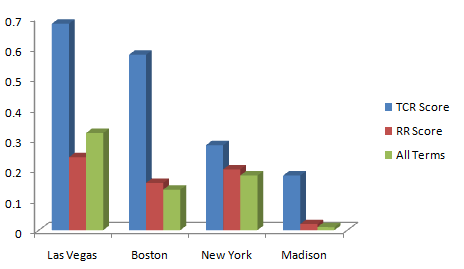
\includegraphics[scale=0.6]{Acc.png}
\caption{Accuracy}
\end{minipage}
\begin{minipage}{.5\linewidth}
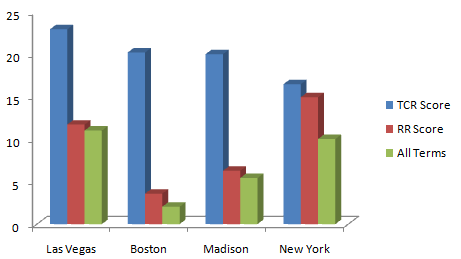
\includegraphics[scale=0.6]{NDCG.png}
\caption{DCG at 5}
\end{minipage}
\end{figure}

\begin{figure}[h!]
\begin{minipage}{.5\linewidth}
\centering
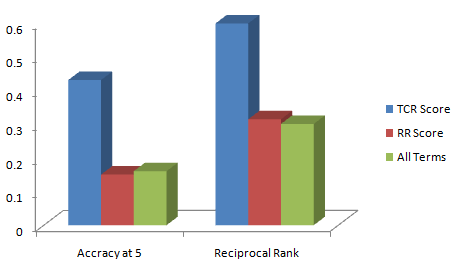
\includegraphics[scale=0.6]{Avg.png}
\caption{Average Accuracy at 5 and Average Reciprocal Rank}
\end{minipage}
\begin{minipage}{.5\linewidth}
\centering
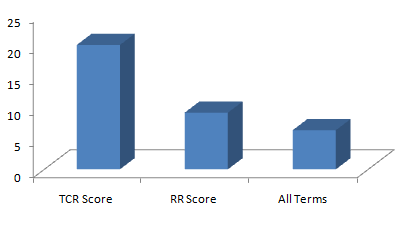
\includegraphics[scale=0.6]{AvgNDCG-2.png}
\caption{Average DCG}
\end{minipage}
\end{figure} 

\section{Result}
The project dealt with businesses provided in the Yelp data. For efficient web indexing, business, reviews, user and tip parts of the data were used. We made an effort to provide search results to a user that are not only pertinent to the query but are also accessible to the user in terms of the location.
We found that the TCR-score ranking performed best for our query set. The average DCG at 5 was
As part of the future work, we would scale up the system to incorporate bigger dataset and perform semantic analysis of the query.

\vspace{40mm}








\bibliographystyle{IEEEtran}      
\bibliography{sample}


\end{document}